%%%%%%%%%%%%%%%%%%%%%%%%%%%%%%%%%%%%%%%%%%%%%%%%%%%%%%%%%%%%%%%%%%%%%%%%%%%%%%%%%%%%%%%
%%%%%%%%%%%%%%%%%%%%%%%%%%%%%%%%%%%%%%%%%%%%%%%%%%%%%%%%%%%%%%%%%%%%%%%%%%%%%%%%%%%%%%%
% 
% This top part of the document is called the 'preamble'.  Modify it with caution!
%
% The real document starts below where it says 'The main document starts here'.

\documentclass[12pt]{article}

\usepackage{amssymb,amsmath,amsthm}
\usepackage[top=1in, bottom=1in, left=1.25in, right=1.25in]{geometry}
\usepackage{fancyhdr}
\usepackage{enumerate}
\usepackage{listings}
\usepackage{graphicx}
% Comment the following line to use TeX's default font of Computer Modern.
\usepackage{times,txfonts}

\newtheoremstyle{homework}% name of the style to be used
  {18pt}% measure of space to leave above the theorem. E.g.: 3pt
  {12pt}% measure of space to leave below the theorem. E.g.: 3pt
  {}% name of font to use in the body of the theorem
  {}% measure of space to indent
  {\bfseries}% name of head font
  {:}% punctuation between head and body
  {2ex}% space after theorem head; " " = normal interword space
  {}% Manually specify head
\theoremstyle{homework} 

% Set up an Exercise environment and a Solution label.
\newtheorem*{exercisecore}{Exercise \@currentlabel}
\newenvironment{exercise}[1]
{\def\@currentlabel{#1}\exercisecore}
{\endexercisecore}

\newcommand{\localhead}[1]{\par\smallskip\noindent\textbf{#1}\nobreak\\}%
\newcommand\solution{\localhead{Solution:}}

%%%%%%%%%%%%%%%%%%%%%%%%%%%%%%%%%%%%%%%%%%%%%%%%%%%%%%%%%%%%%%%%%%%%%%%%
%
% Stuff for getting the name/document date/title across the header
\makeatletter
\RequirePackage{fancyhdr}
\pagestyle{fancy}
\fancyfoot[C]{\ifnum \value{page} > 1\relax\thepage\fi}
\fancyhead[L]{\ifx\@doclabel\@empty\else\@doclabel\fi}
\fancyhead[C]{\ifx\@docdate\@empty\else\@docdate\fi}
\fancyhead[R]{\ifx\@docauthor\@empty\else\@docauthor\fi}
\headheight 15pt

\def\doclabel#1{\gdef\@doclabel{#1}}
\doclabel{Use {\tt\textbackslash doclabel\{MY LABEL\}}.}
\def\docdate#1{\gdef\@docdate{#1}}
\docdate{Use {\tt\textbackslash docdate\{MY DATE\}}.}
\def\docauthor#1{\gdef\@docauthor{#1}}
\docauthor{Use {\tt\textbackslash docauthor\{MY NAME\}}.}
\makeatother

% Shortcuts for blackboard bold number sets (reals, integers, etc.)
\newcommand{\Reals}{\ensuremath{\mathbb R}}
\newcommand{\Nats}{\ensuremath{\mathbb N}}
\newcommand{\Ints}{\ensuremath{\mathbb Z}}
\newcommand{\Rats}{\ensuremath{\mathbb Q}}
\newcommand{\Cplx}{\ensuremath{\mathbb C}}
%% Some equivalents that some people may prefer.
\let\RR\Reals
\let\NN\Nats
\let\II\Ints
\let\CC\Cplx

%%%%%%%%%%%%%%%%%%%%%%%%%%%%%%%%%%%%%%%%%%%%%%%%%%%%%%%%%%%%%%%%%%%%%%%%%%%%%%%%%%%%%%%
%%%%%%%%%%%%%%%%%%%%%%%%%%%%%%%%%%%%%%%%%%%%%%%%%%%%%%%%%%%%%%%%%%%%%%%%%%%%%%%%%%%%%%%
% comment 
% The main document start here.

% The following commands set up the material that appears in the header.
\doclabel{Math 426: Homework 1 (Part B)}
\docauthor{Stefano Fochesatto}
\docdate{\today}

\begin{document}
\textbf{Part B (Matlab Tutorial)}


\begin{exercise}{2} With the matrices and vectors,
\begin{equation*}
  A = 
  \begin{pmatrix}
    10 && -3 \\
    4 && 2 
  \end{pmatrix},
  B = 
  \begin{pmatrix}
    1 && 0 \\
    -1 && 2 
  \end{pmatrix},
    v = 
  \begin{pmatrix}
    1 \\
    2 
  \end{pmatrix},
    w = 
  \begin{pmatrix}
    1 \\
    1 
  \end{pmatrix},
\end{equation*}
 compute the following both by hand and in MATLAB. For the MATLAB computations use the diary command to record your session.
\begin{enumerate}
  \item[a.] $v^{T}w$\\\\
  \textbf{Solution:} 
  
  \begin{align*}
    v^{T}w &=
    \begin{pmatrix}
      1&&2 \\
    \end{pmatrix}
    \begin{pmatrix}
      1 \\
      1
    \end{pmatrix},\\
    &=
    (1*1)+(1*2),\\
    &= 3.
  \end{align*}
  
  \item[b.] $vw^{T}$\\\\
  \textbf{Solution:} 

  \begin{align*}
    vw^{T} &=
    \begin{pmatrix}
      1 \\
      2
    \end{pmatrix}
    \begin{pmatrix}
      1 \\
      1
    \end{pmatrix},\\
    &=
    \begin{pmatrix}
      1*1 && 1*1 \\
      2*1 && 2*1
    \end{pmatrix},
    \\
    &= \begin{pmatrix}
      1 && 1 \\
      2 && 2
    \end{pmatrix}.
  \end{align*}
  
  \item[c.] $Av$\\\\
  \textbf{Solution:}

  \begin{align*}
    Av &=
    \begin{pmatrix}
      10 && -3 \\
      4 && 2 
    \end{pmatrix}
    \begin{pmatrix}
      1 \\
      2
    \end{pmatrix},\\
    &=
    \begin{pmatrix}
      (10*1) + (-3*2) \\
      (4*1) + (2*2)
    \end{pmatrix},
    \\
    &= \begin{pmatrix}
      4 \\
      8
    \end{pmatrix}.
  \end{align*}






  \item[d.] $A^{T}v$\\\\
  \textbf{Solution:}

  \begin{align*}
    A^{T}v &=
    \begin{pmatrix}
      10 && 4 \\
      -3 && 2 
    \end{pmatrix}
    \begin{pmatrix}
      1 \\
      2
    \end{pmatrix},\\
    &=
    \begin{pmatrix}
      (10*1) + (4*2) \\
      (-3*1) + (2*2)
    \end{pmatrix},
    \\
    &= \begin{pmatrix}
      18 \\
      1
    \end{pmatrix}.
  \end{align*}




  \item[e.] $AB$\\\\
  \textbf{Solution:}

  \begin{align*}
    AB &=
    \begin{pmatrix}
      10 && -3 \\
      4 && 2 
    \end{pmatrix}
    \begin{pmatrix}
      1 && 0 \\
      -1 && 2 
    \end{pmatrix},
    \\
    &=
    \begin{pmatrix}
      (10*1) + (-3*-1) && (10*0) + (-3*2) \\
      (4*1) + (2*-1) && (4*0) + (2*2)
    \end{pmatrix},
    \\
    &= \begin{pmatrix}
      13 && -6 \\
      2 && 4 
    \end{pmatrix}.
  \end{align*}

  \item[f.] $BA$\\\\
  \textbf{Solution:}

  \begin{align*}
    BA &=
    \begin{pmatrix}
      1 && 0 \\
      -1 && 2 
    \end{pmatrix}
    \begin{pmatrix}
      10 && -3 \\
      4 && 2 
    \end{pmatrix},
    \\
    &=
    \begin{pmatrix}
      (1*10) + (0*4) && (1*-3) + (0*2) \\
      (-1*10) + (2*4) && (-1*-3) + (2*2)
    \end{pmatrix},
    \\
    &= \begin{pmatrix}
      10 && -3 \\
      -2 && 7 
    \end{pmatrix}.
  \end{align*}


  \item[g.] $A^2$\\\\
  \textbf{Solution:}
  
  \begin{align*}
    AA &=
    \begin{pmatrix}
      10 && -3 \\
      4 && 2 
    \end{pmatrix}
    \begin{pmatrix}
      10 && -3 \\
      4 && 2 
    \end{pmatrix},
    \\
    &=
    \begin{pmatrix}
      (10*10) + (-3*4) && (10*-3) + (-3*2) \\
      (4*10) + (2*8) && (4*-3) + (2*2)
    \end{pmatrix},
    \\
    &= \begin{pmatrix}
      88 && -36 \\
      48 && -8 
    \end{pmatrix}.
  \end{align*}

  \item[h.] $By = w$\\\\
  \textbf{Solution:}

  \begin{align*}
    By &= w\\
    \begin{pmatrix}
      1 && 0 \\
      -1 && 2 
    \end{pmatrix} 
    \begin{pmatrix}
      y_1 \\
      y_2 
    \end{pmatrix}
    &=
    \begin{pmatrix}
      1 \\
      1 
    \end{pmatrix},\\
    \begin{pmatrix}
      y_1 \\
      y_2 
    \end{pmatrix}
    &=
    \frac{1}{(1*2)-(0*-1)}
    \begin{pmatrix}
      2 && 0 \\
      1 && 1 
    \end{pmatrix}
    \begin{pmatrix}
      1 \\
      1 
    \end{pmatrix}\\
    \begin{pmatrix}
      y_1 \\
      y_2 
    \end{pmatrix}
    &=
    \begin{pmatrix}
      1 && 0 \\
      \frac{1}{2} && \frac{1}{2} 
    \end{pmatrix}
    \begin{pmatrix}
      1 \\
      1 
    \end{pmatrix}\\
    \begin{pmatrix}
      y_1 \\
      y_2 
    \end{pmatrix}
    &=
    \begin{pmatrix}
      1 \\
      1 
    \end{pmatrix}
  \end{align*}

  \item[i.] $Ax = v$\\\\
  \textbf{Solution:}       
  \begin{align*}
    Ax &= v\\
    \begin{pmatrix}
      10 && -3 \\
      4 && 2 
    \end{pmatrix} 
    \begin{pmatrix}
      x_1 \\
      x_2 
    \end{pmatrix}
    &=
    \begin{pmatrix}
      1 \\
      2 
    \end{pmatrix},\\
    \begin{pmatrix}
      x_1 \\
      x_2 
    \end{pmatrix}
    &=
    \frac{1}{(10*2)-(-3*4)}
    \begin{pmatrix}
      2 && 3 \\
      -4 && 10 
    \end{pmatrix}
    \begin{pmatrix}
      1 \\
      2 
    \end{pmatrix}\\
    \begin{pmatrix}
      x_1 \\
      x_2 
    \end{pmatrix}
    &=
    \begin{pmatrix}
      \frac{2}{32} && \frac{3}{32} \\
      \frac{-4}{32} && \frac{10}{32} 
    \end{pmatrix}
    \begin{pmatrix}
      1 \\
      2 
    \end{pmatrix}\\
    \begin{pmatrix}
      x_1 \\
      x_2 
    \end{pmatrix}
    &=
    \begin{pmatrix}
      \frac{1}{4} \\
      \frac{1}{2} 
    \end{pmatrix}
  \end{align*} 


\end{enumerate}
\end{exercise}
\vspace{1in}







\begin{exercise}{4} Use MATLAB to print a table of values $x$, $sin x$, and $cos x$, for,
  \begin{equation*}
    x = 0, \frac{\pi}{6}, \frac{2\pi}{6}, \ldots , 2\pi.
  \end{equation*}
  Label the columns of your table.\\\\
\textbf{Solution:}
\lstinputlisting{ex4}



\end{exercise}
\vspace{1in}

\begin{exercise}{5}  Download the file $plotfunction1.m$ from the book's web page and execute it. This should produce the two plots on the next page. 
  The top plot shows the function $f(x) = 2cos(x) - e^{x}$ for $-6 \le x \le 3$, and the from this plot it appears that $x$ has three roots in this interval. 
  The bottom plot is a zoomed view near one of these roots, showing that $x$ has a root neat $x = -1.454$. 
  Note the different vertical scale as well as the different horizontal scale of this plot. 
  Not also that when we zoo, in on this function it looks neatly linear over this short interval. This will be important when we study numerical methods for approximating roots.\\\\


\begin{enumerate}

  \item [\textbf{a.}] Modify the script so that the bottom plot shows a zoomed view near the leftmost root. Write an estimate of the value of this root to at least 3 decimal places.
  You may find it useful to first use the zoom feature in MATLAB to see approximately where the root is and then to choose your axis command for the second plot appropriately.\\\\
  \textbf{Solution:} 
  \vspace{1in}
  \lstinputlisting{plotfunction1.m}
  \begin{center}
    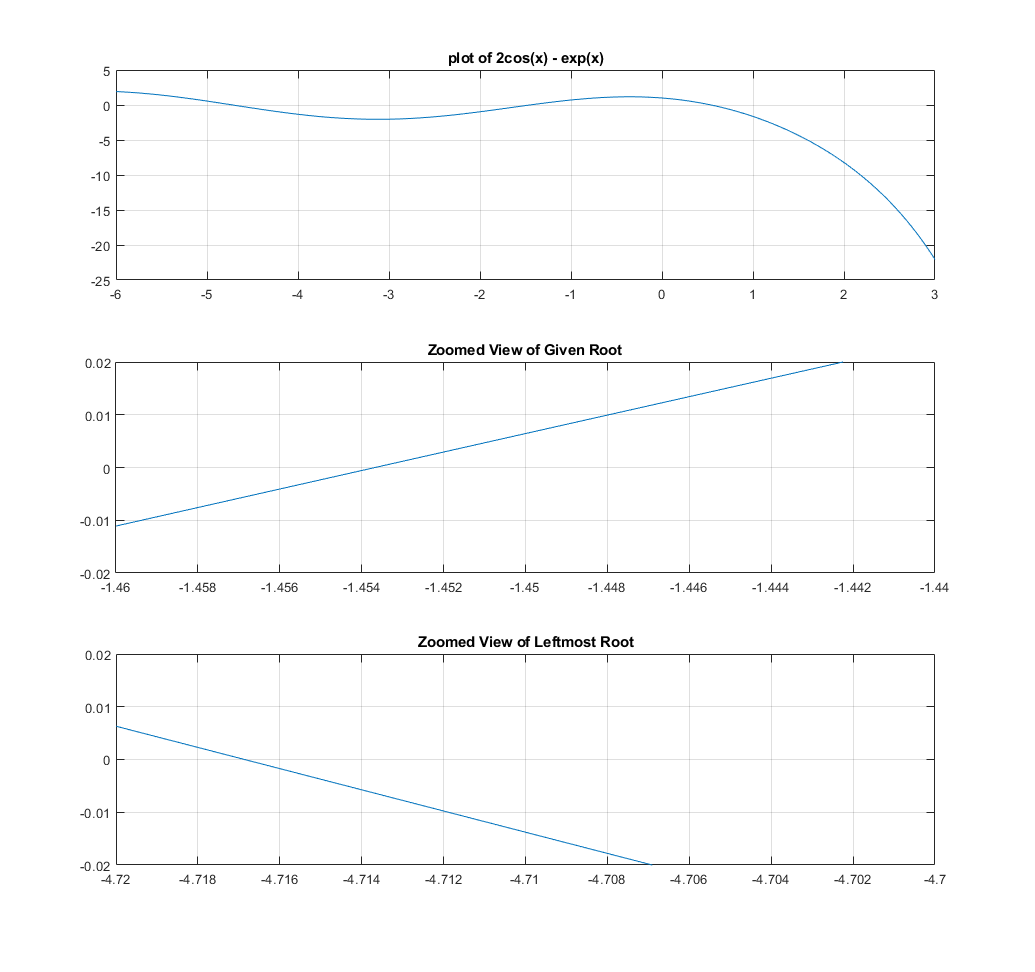
\includegraphics[width=\textwidth]{plotfunction.png}
  \end{center}
  The leftmost root for the function $f(x) = 2cos(x) - e^{x}$ on the interval $-6 \le x \le 3$ is at approximately $x = -4.717$.




  \item [\textbf{b.}] Edit the script from part a to plot the function,
  \begin{equation*}
    f(x) = \frac{4x sin(x) - 3}{2 + x^2}
  \end{equation*}
  over the range $ 0 \le x \le 4$ and also plot a zoomed view neat the leftmost root.
   Write an estimate of the value of the root from the plots that is accurate to 3 decimal places.
  Note that once you have defined the vector $x$ properly, you will need to use appropriate components multiplication and division to evaluate this expression.\\\\
  \textbf{Solution:} 
  
  \lstinputlisting{plotfunction2.m}
  \begin{center}
    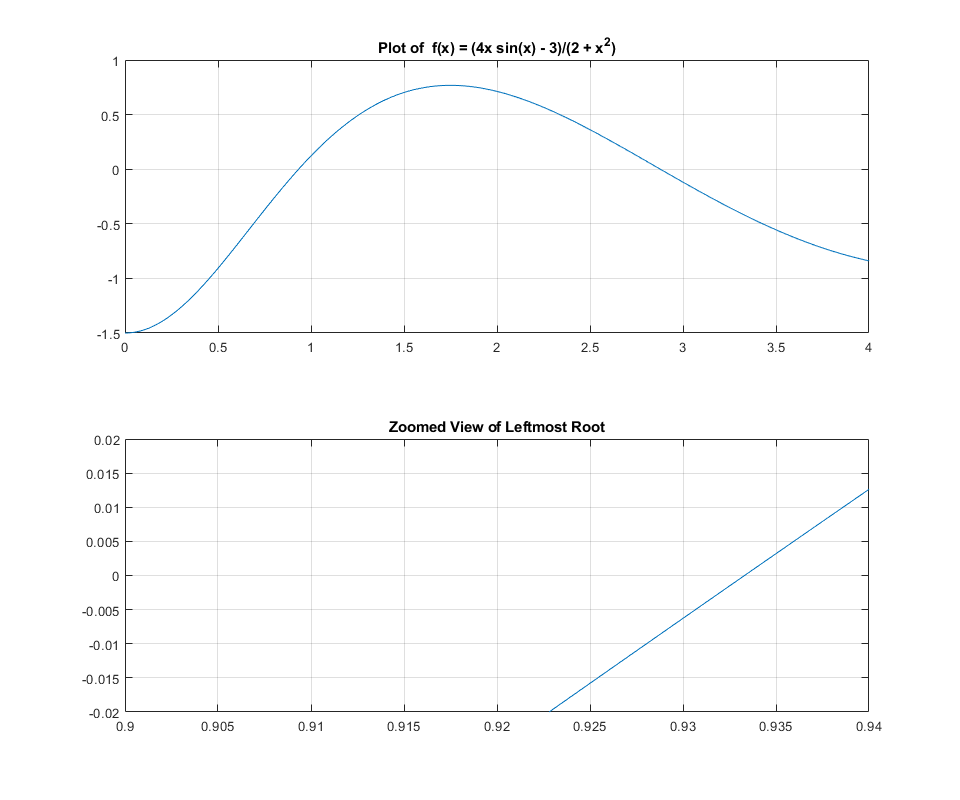
\includegraphics[width=\textwidth]{plotfunction2.png}
  \end{center}
  
  The leftmost root for the function $f(x) = \frac{4x sin(x) - 3}{2 + x^2}$ on the interval $-6 \le x \le 3$ is at approximately $x = .933$.
  \end{enumerate}

\end{exercise}
\vspace{1in}







\begin{exercise}{7} Use MATLab to plot the circles,
  \begin{align*}
    (x - 2)^2 + (y - 2)^2 &= 2,\\
    (x - 2.5)^2 + (y)^2 &= 3.5,
    \end{align*}
  and zoom in on the plot to determine approximately where the circles intersect.
\textbf{Solution:}

\lstinputlisting{circle.m}
\begin{center}
  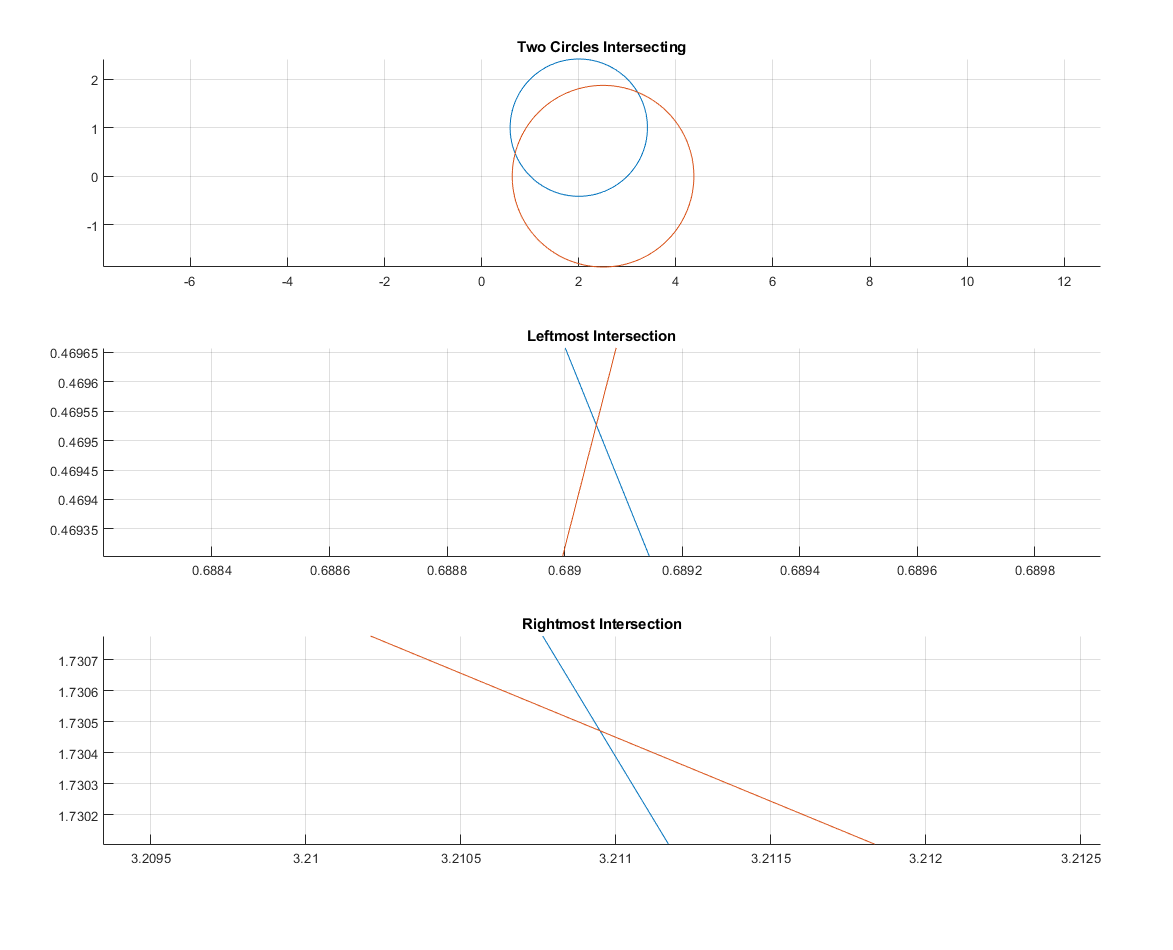
\includegraphics[width=\textwidth]{circle.png}
\end{center}
The leftmost intersection is is at approximately $(.691,.454)$ and the rightmost intersection is at approximately $(3.212, 1.730)$.
\end{exercise}
\vspace{1in}



\begin{exercise}{9} Create a $5 x 5$ magic square and verify using the sum command in Matlab that the sums of the columns, rows and diagonals are equal.\\\\
\textbf{Solution:} 
\lstinputlisting{ex9}
\end{exercise}
\vspace{1in}



\end{document}

